\chapter{Content of DVD}
This work contains a DVD with following structure:
\begin{itemize}
	\item \textbf{bin/} folder with a self extracting archive containing compiled application for Windows along with required libraries.
	\item \textbf{doc/} folder containing source code documentation generated by Doxygen. 
	\item \textbf{latex/} folder containing \LaTeX\ source codes for generating text of this thesis.
	\item \textbf{source/} folder containing source codes for building the application. Refer to the included \textbf{README.md} for instructions on how to build the application.
\end{itemize}
The content of the archive with compiled application is following:
\begin{itemize}
	\item \textbf{data/} folder containing EEG data in the EDF format for testing purposes.
	\item \textbf{electrodes/} folder which contains \texttt{default.elmap} specifying default electrode placement and \texttt{electrodes.obj} providing 3D electrode positions. 
	\item \textbf{licenses/} folder containing licenses for used libraries, EEG data and models.
	\item \textbf{models/} folder containing mesh models.
	\item \textbf{platforms/} folder with Qt libraries specific for Windows platform.
	\item \textbf{shaders/} folder with GLSL source codes that are compiled during run-time by the application.
	\item \textbf{bav.exe} -- the application executable.
	\item \textbf{.dll files} -- dynamic libraries required by the application.
	\item \textbf{MANUAL.txt} -- short manual describing basic interaction with the application.
\end{itemize}

\chapter{Image of Graphical User Interface}
\begin{figure}[htb]
	\centering
	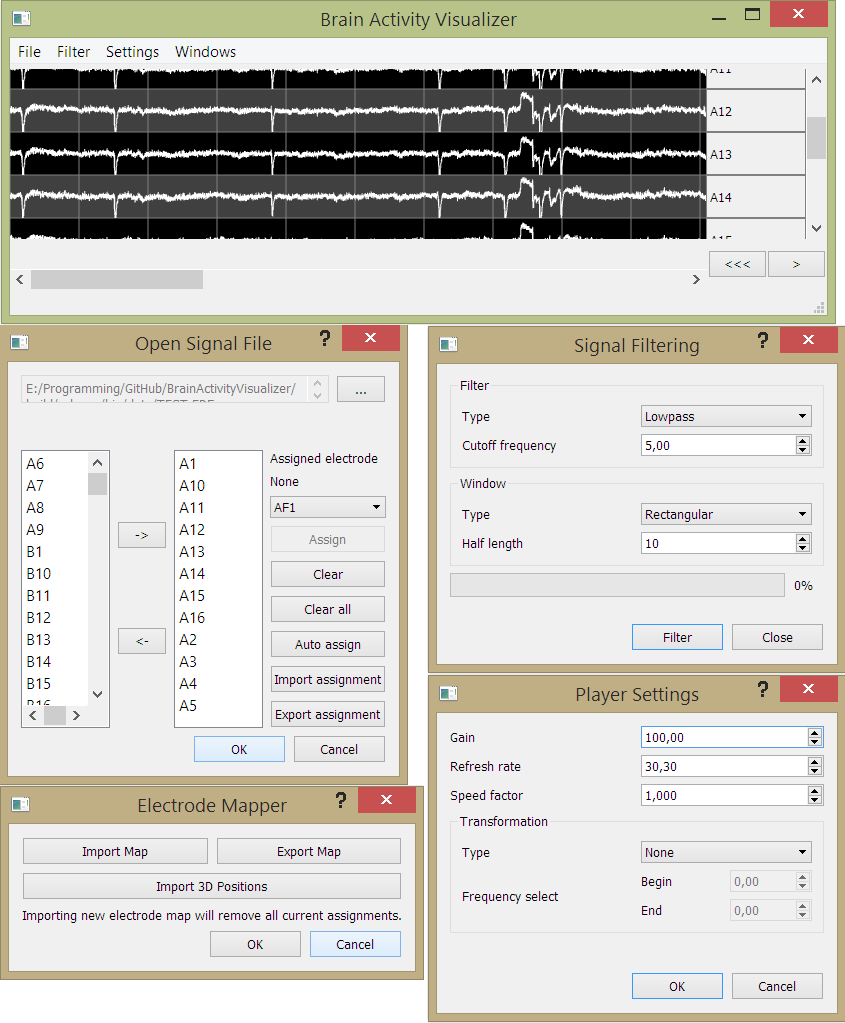
\includegraphics[width=0.85\linewidth]{fig/gui.png}
\end{figure}

\chapter{Signal Filtering Tests}
The signal module which encompasses signal processing methods was tested against the MATLAB software to check the validity of implementation. First, a random signal with  $10000$ samples was generated. The signal was then filtered by the testing executable \textbf{sigTest.exe}. The testing executable is generated during build if the project was configured with \texttt{-DTEST\_PROJ=true}. The filtering was done in multiple configuration which are listed in table below.

\begin{table}[!h]
	\centering
	\label{t:filterCfg}
	\begin{tabular}{|c|c|c|c|c|}	
		\hline Filter & Window & Order & Cutoff frequency & Filename \\ 
		\hline Low-pass & Hamming & 10 & 5 & low5Hamm5 \\ 
		\hline Low-pass & Hamming & 10 & 10 & low10Hamm5 \\ 
		\hline Low-pass & Hamming & 20 & 5 & low5Hamm10 \\ 
		\hline Low-pass & Hamming & 20 & 10 & low10Hamm10 \\ 
		\hline Low-pass & Blackman & 10 & 5 & low5Black5 \\ 
		\hline Low-pass & Blackman & 10 & 10 & low10Black5 \\ 
		\hline Low-pass & Blackman & 20 & 5 & low5Black10 \\ 
		\hline Low-pass & Blackman & 20 & 10 & low10Black10 \\ 
		\hline High-pass & Hamming & 10 & 50 & high50Hamm5 \\ 
		\hline High-pass & Hamming & 10 & 100 & high100Hamm5 \\ 
		\hline High-pass & Hamming & 20 & 50 & high50Hamm10 \\ 
		\hline High-pass & Hamming & 20 & 100 & high100Hamm10 \\ 
		\hline High-pass & Blackman & 10 & 50 & high50Black5 \\ 
		\hline High-pass & Blackman & 10 & 100 & high100Black5 \\ 
		\hline High-pass & Blackman & 20 & 50 & high50Black10 \\ 
		\hline High-pass & Blackman & 20 & 100 & high100Black10 \\ 
		\hline 
	\end{tabular}
	\caption{Tested filter configurations}
\end{table}

Each configuration produced single output file with the filtered signal. This file was read by a MATLAB script and compared to the result of filtering using MATLAB filters in the same configuration. The maximum and average deviation was calculated and printed to output. The difference between signals filtered by testing executable and MATLAB in all configurations was marginal and can be attributed to floating point errors.

\chapter{Code metrics}
\vfill
\begin{table}[!h]
	\centering
	\label{t:codeMetrics}
	\begin{tabular}{|l|c|}
		\hline Files &  89 \\ 
		\hline Lines of code & 7517 \\
		\hline Percent of comments & 11.5\% \\ 
		\hline Statements & 3436 \\ 
		\hline Class definitions & 47 \\ 
		\hline Methods per class & 7.98 \\ 
		\hline Statements per method & 5.2 \\ 
		\hline Maximum depth & 6 \\
		\hline Average depth & 1.12 \\
		\hline 
	\end{tabular} 
	\caption{Code metrics}
\end{table}
\vfill
%\chapter{Manual}
